
 \documentclass[12pt]{article} % Документ принадлежит классу article, а также будет печататься в 12 пунктов.
\usepackage[russian]{babel} % Пакет поддержки русского языка
\usepackage{amsmath} %пакет формул
\title{Теория Алгоритма} % Заглавие документа
\usepackage{alltt}
\date{\today} % Дата создания
\parindent=1cm
\usepackage{graphicx}
\graphicspath{{pictures/}}
\DeclareGraphicsExtensions{.png}
 \begin{document}
 	\tableofcontents
 	\newpage
 	\section{Фурмолировка задачи}
 	
 	\section{Условия упрощения алгоритма}
 	\subsection{Фурмалировка условий упрощения алгоритма}
 	\hspace*{1cm}Так как мы пишем программу, что бы облегчить себе задачу, будем искать куда поставить почтамт методом переюора. Но перебор длжен быть организован так, что:\\
 	\hspace*{5mm}1. Точек куда можно поставить почтамт конечно, и их количество должно быть \(a<\text{n}<b\) ($10^5<n<10^6$).\\
 	\hspace*{5mm}2. Для каждой точки можно определить скалярную функцию входных данных(центры активности(далее ЦА), зоны запрета полета(далее NFZ), населенности в районе).\\
 	\hspace*{5mm}3. Входные данные должны быть осмысленны.
 	\subsection{Уточним первое условие}
 	\hspace*{10mm}Теперь определим \(a\), \(b\). Переменая $a$ отвечает за то что бы не упрастить задачу до одной точки. Я думаю $a$ должно быть таким, что растояние между точками меньше 100метров. Площадь Маската 3500 $km^2$ откуда получаем $a\approx \cfrac{35\cdot 10^8}{100^2} =35 \cdot 10^4   $, а если учесть что 1/3 маската это малонаселенные горы получаем $a \approx 10^5$. Значение $b$ можно определить из времени выполнения программы. Дадим напрмер на алгорим 10 минут. количество операций которое можно провести за это время можн опонять из такой программы:\\
 	\begin{alltt}
 		\textit{1 import datetime
 		2 t = datetime.datetime.now()
 		3 i = 0
 		4 while (datetime.datetime.now() - t).seconds < 30:
 		5     i += 1
 		6 print(i * 20)}
 	\end{alltt}
 	Вывод программы зависит от устройства на котором она запущена. У меня выдала $792801540$ или  примерно $8000 \cdot 10^5$ и если на одну точку брать хотя бы 800 простых операций получаем $b \approx10^6$ \par
 	Итак первое условие $10^5<n<10^6$
 	\subsection{Уточним второе условие}
 	\hspace*{10mm} Для начала определим еще один важный фактор. Наша программа раставляет пачтамты последовательно и от наиболее загруженного к наименее загруженому, отсюда получаем ситуацию: стоит почтамт и не так далеко находится ЦА. Мы конечно хотим поставить пачтамт рядом с ЦА, но тут уже стоит один. Отсюда следствие: функция должна учитывать так же уже поставленные пачтамты. \\
 	\hspace*{5mm}2.1 функция должна опираться на уже поставленные пачтамты 
 	\subsection{Уточним третье условие}
 	\hspace*{1cm}Проблема в том, что точных данных по населенности у нас нет. Поэтому мы пришли к упращению: Маскат распередлен на регионы, где население распределено равномерно. Если внутри региона видно сильное разделение, то мы искуственно разделим этот регион на "подрегионы" и пделим население так, как нам покажется правильным, что бы население в "подрегионах" было $\pm$ равномерно.\par
 	То-есть все данные должны быть проработаны на правдивость и поэтому результат программы должен быть так же осознан(должен подвергнуться критике со стороны человека) 
 	\section{Входные даные}
 	\subsection{Область обработки входных данных}
 	\hspace*{1cm} Как мы понимаем, люди не будут использовать почтамат если он находится в 10km от их дома. Так же очевидно, что чем дальше почтамт от их дома, тем меньше они будут им пользоваться. Я бы взял растояние до 2km и функцию от растояния $f(R)\sim\frac{1}{R^2}$ или даже $f(R)\sim\frac{1}{R^3}$.\par
 	 Так же с ЦА. люди из ЦА пойдут к пачтамту только если он очень близко, посколько в бизнес центре или складе время-деньги, а в магазинах люди веселяться так что не готовы идти долеко в этом и смысл торговых центров. Отсюда радиус < 500m а $f(R)\sim \frac{1}{R^3}$. \par 
 	 NFZ будут обрабатаваться просто как точки, где поставить пачтамты нельзя. 
 	 \subsection{Обработка входных даных}
 	 \hspace*{1cm}На вход алгоритм получит точки(определяющие регионы), насеоенность регионов, точки(определяющие ЦА), рейтинг(рейтинг ЦА который создан субьективно, но пропорцианален количеству посылок, отправляемых из ЦА).\par
 	 Мы хотим их привести к данным, которые проще обрабатывать. Поэтому привратим регионы в набор точек каждой из которых будет присвоено значение населености.\\
 	 \textbf{Проблема: }Регионы - не всегда выпуклые многоугольники занчит определить принадлежит ли точка многоугольнику нельзя просто проверив принадлежит ли точка всем полуплоскостям образованными гранями. \par
 	 \textbf{Решение: }Изменим многоугольник вырезая вершины так, что он станет выпуклым. Получим: \\
 	 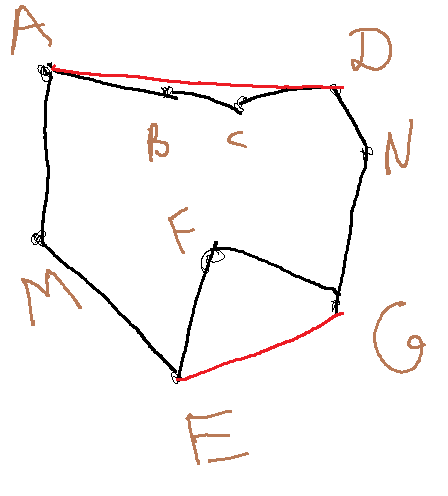
\includegraphics[scale=0.7]{1}\\
 	 в даном случае остается проверить для точки $U = (x, y), \; U \in ADGEM \cap U \notin FEG \cap U \notin ABCD$. \par
 	 Как же найти такие EFG? Как мы знаем уравнение прямой выглядит так: $\cfrac{x-x_1}{x_2 - x_1} = \cfrac{y-y_1}{y_2 -y_1}$. Теперь как определить что точка лежит справа? Можно просто посмоттеть где прямая через т U пересекает ось X например:\\
 	 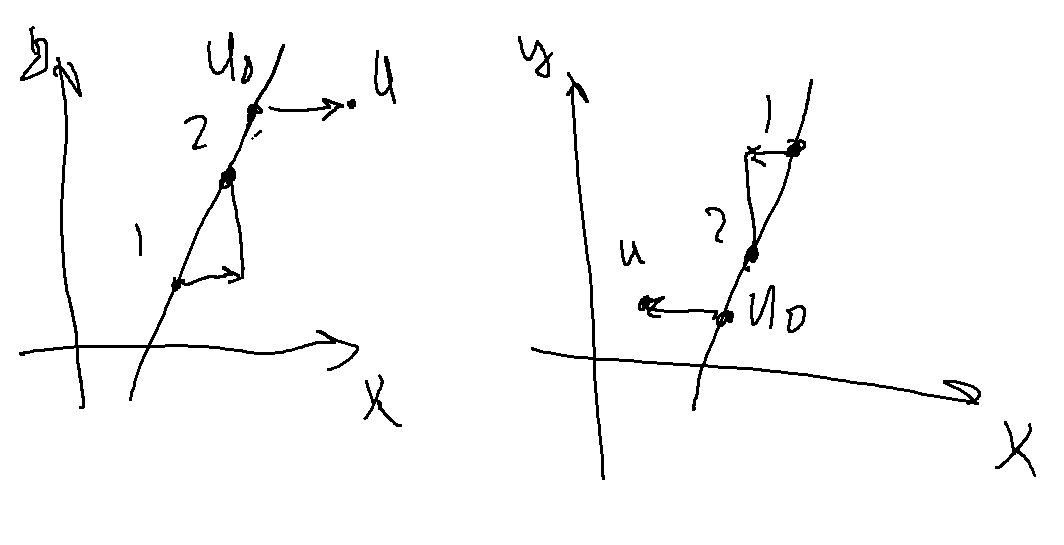
\includegraphics[scale=0.9]{2}\\
 	 \hspace*{1cm}Подставим y от U в уравнение получим:$x_3 =\cfrac{(y_U-y_1)(x_2 - x_1)}{y_2 -y_1} + x_1 $ тогда $U_0 = (x_3, y_U)$ тогда если точка 2 лежит правее точки 1 то и U должна лежать правее точки $U_0$ получаем по знаку $\cfrac{(y_U-y_1)(x_2 - x_1)}{y_2 -y_1}\equiv x_2 - x_1$ просокращав получим $\cfrac{y_U-y_1}{y_2 -y_1} > 0$. Случай $U \in \cfrac{x-x_1}{x_2 - x_1} = \cfrac{y-y_1}{y_2 -y_1}$ нужно расмотреть отдельно но пусть в таком счучае будем считать, что принадлежит.
 	 \subsection{Итоговые Входные даные}
 	 Итак мы упрастили ввод до точек каждой из которой принадлежит ярлык ЦА или просто регион и какя то цифра хорактерезующая количество отправок.
 	 \section{Алгоритм}
 \end{document}